% Drawing 74/04-3 -- folder 74, batch 04, archive page 61 (PDF page 62).
% Transcription: figure à neuf sommets $i, j?, k, p, q, r, s, t, u$ : un rectangle $i\,p\,q\,k$ coupé par des traits pleins et pointillés, l'arête $ip$ marquée $(a)$, et une colonne verticale $s, t, u$ reliée en $u$ aux sommets $p$, $q$, $r$.
% Kind: figure on nine vertices. Method 2 (schematic redraw from the facsimile). Status: partial.
% Notes: Left column i, j?, k; right column p, q, r; the column s, t, u at the right, u joined to the right column. Edge ip marked (a). Solid and dashed strokes inside the rectangle are drawn as seen; which vertices the inner strokes join is partly a reading. The transcription's « rectangle i p q k » has, on the page, p, q, r down the right side.
% Coordinates: 1 unit = 1 mm = 1/100 of the crop width (bbox in page fractions: [0.25, 0.73, 0.48, 0.88]).
% Redrawn by Claude (claude-opus-5-5), issue #73, 2026-11-07; not checked by a human; not compiled (no TeX in the session).
% Rights: reproduces part of the work -- behind RENDER_TRANSCRIPTS, never published by itself.
\documentclass[tikz,border=3pt]{standalone}
\usepackage{amsmath,amssymb}
\usetikzlibrary{patterns,arrows.meta}
\tikzset{pencil/.style={black!45}, struck/.style={black!35}, mark/.style={circle,draw,inner sep=1.3pt}, pt/.style={circle,fill,inner sep=0.9pt}, opt/.style={circle,draw,fill=white,inner sep=1.1pt}}
\begin{document}
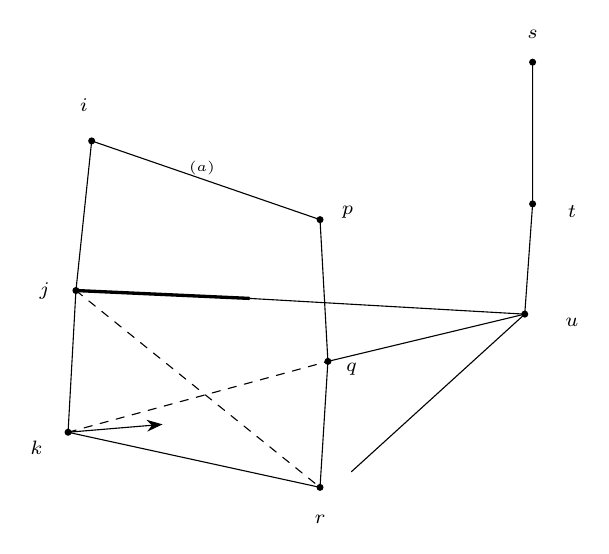
\begin{tikzpicture}[x=1mm,y=1mm,line cap=round,line join=round,font=\scriptsize]
\draw (16,-20) -- (45,-30);
\draw (16,-20) -- (14,-39) -- (13,-57);
\draw (45,-30) -- (46,-48) -- (45,-64);
\draw (13,-57) -- (45,-64);
\draw[very thick] (14,-39) -- (36,-40);
\draw (72,-10) -- (72,-28) -- (71,-42);
\draw (36,-40) -- (71,-42);
\draw (46,-48) -- (71,-42);
\draw (49,-62) -- (71,-42);
\draw[dashed] (13,-57) -- (46,-48);
\draw[dashed] (14,-39) -- (45,-64);
\draw[-{Stealth[length=2mm]}] (13,-57) -- (25,-56);
\node[pt] at (16,-20) {};
\node[pt] at (14,-39) {};
\node[pt] at (13,-57) {};
\node[pt] at (45,-30) {};
\node[pt] at (46,-48) {};
\node[pt] at (45,-64) {};
\node[pt] at (72,-10) {};
\node[pt] at (72,-28) {};
\node[pt] at (71,-42) {};
\node[inner sep=1pt] at (15,-15.5) {\scriptsize $i$};
\node[inner sep=1pt] at (10,-39) {\scriptsize $j$};
\node[inner sep=1pt] at (9,-59) {\scriptsize $k$};
\node[inner sep=1pt] at (48.5,-29) {\scriptsize $p$};
\node[inner sep=1pt] at (49,-49) {\scriptsize $q$};
\node[inner sep=1pt] at (45,-68) {\scriptsize $r$};
\node[inner sep=1pt] at (72,-6.5) {\scriptsize $s$};
\node[inner sep=1pt] at (77,-29) {\scriptsize $t$};
\node[inner sep=1pt] at (77,-43) {\scriptsize $u$};
\node[inner sep=1pt] at (30,-23.5) {\tiny $(a)$};
\end{tikzpicture}
\end{document}
